% One-page A4 poster. Compile with pdfLaTeX.
% Keep CUHK-Shenzhen.jpg and registration_QR_12_2026.png in this folder.
\documentclass[11pt,a4paper]{article}
\usepackage[utf8]{inputenc}
\usepackage[T1]{fontenc}
\usepackage[scaled=.98]{helvet}
\renewcommand{\familydefault}{\sfdefault}
\usepackage[a4paper,margin=0pt]{geometry}
\usepackage{xcolor,graphicx,tikz,ragged2e,microtype}
\usepackage[hidelinks]{hyperref}

\definecolor{navy}{HTML}{003366}
\definecolor{deepnavy}{HTML}{102A43}
\definecolor{accent}{HTML}{276EA3}
\definecolor{ink}{HTML}{233242}
\definecolor{muted}{HTML}{536577}
\definecolor{panel}{HTML}{F0F5FA}
\definecolor{lineblue}{HTML}{CFDEE9}
\hypersetup{
  pdftitle={Frontiers of AI Mathematical Reasoning: Capabilities, Limitations, and Paths to Improvement},
  pdfauthor={Workshop Organising Committee},
  pdfsubject={Academic-industry workshop at CUHK-Shenzhen, 4 December 2026},
  pdfkeywords={AI, mathematical reasoning, CUHK-Shenzhen, workshop, December 2026}
}
\pagestyle{empty}
\setlength{\parindent}{0pt}
\setlength{\parskip}{0pt}

\newcommand{\RegistrationURL}{https://forms.cloud.microsoft/Pages/ResponsePage.aspx?id=eouJ5YecS0qyKi3z81XgHrqXUbSx0-BNiJA8Po9fctVUQTVaR0dBVkVWRFNMREcwWko1SjYyUUdVVC4u}

\begin{document}
\noindent
\begin{tikzpicture}[remember picture,overlay]
\begin{scope}[shift={(current page.north west)},x=1mm,y=-1mm,
  every node/.style={inner sep=0pt,outer sep=0pt,anchor=north west}]

% CAMPUS-PHOTO HEADER
\begin{scope}
  \clip (0,0) rectangle (210,84);
  \node at (0,-20) {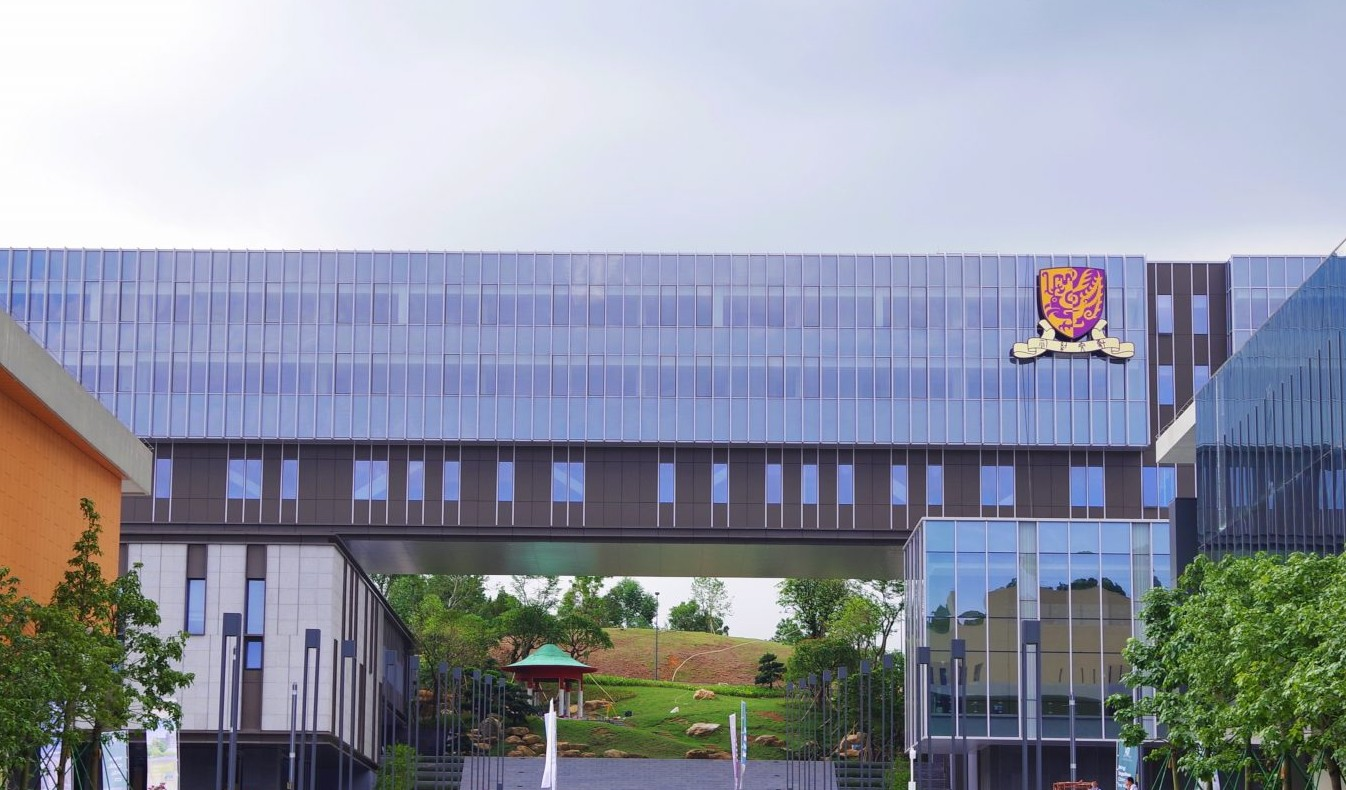
\includegraphics[width=210mm]{CUHK-Shenzhen.jpg}};
  \fill[deepnavy,opacity=.71] (0,0) rectangle (210,84);
\end{scope}
\node[text=white,text width=176mm] at (17,13.5) {
  \fontsize{9.2}{12}\selectfont\bfseries
  \textls[130]{ACADEMIC--INDUSTRY WORKSHOP}
};
\node[text=white,text width=178mm] at (17,26) {
  \fontsize{33.5}{38.5}\selectfont\bfseries\RaggedRight
  Frontiers of AI\\
  Mathematical Reasoning:\par
};
\node[text=white,text width=176mm] at (17,58) {
  \fontsize{16}{20}\selectfont\RaggedRight
  Capabilities, Limitations,\\
  and Paths to Improvement\par
};
\fill[accent] (0,83.3) rectangle (210,84.3);

% WORKSHOP DESCRIPTION -- supplied wording
\node[text=ink,text width=176mm] at (17,99) {
  \fontsize{12}{17}\selectfont\RaggedRight
  An academic--industry workshop bringing together researchers from leading
  AI laboratories and universities to investigate the reasoning capabilities
  of frontier language models, with particular emphasis on open-weight models.\par
};

\node[text=navy,text width=176mm] at (17,127) {
  \fontsize{11.3}{15}\selectfont\bfseries
  The workshop will present:
};

\fill[accent] (19,140) circle (.85);
\node[text=ink,text width=169mm] at (24,137) {
  \fontsize{11.7}{16.3}\selectfont\RaggedRight
  \textbf{Recent industry insights into LLMs for mathematics}, covering
  training data, reinforcement learning, and harness design.\par
};

\fill[accent] (19,161.5) circle (.85);
\node[text=ink,text width=169mm] at (24,158.5) {
  \fontsize{11.7}{16.3}\selectfont\RaggedRight
  \textbf{New results from a large-scale, head-to-head benchmarking study of
  leading models}, highlighting their strengths and limitations.\par
};

\node[text=ink,text width=176mm] at (17,181.5) {
  \fontsize{11.7}{16.3}\selectfont\RaggedRight
  Building on these findings, researchers from academia and industry will
  discuss how to \mbox{collaboratively} improve mathematical reasoning systems and
  identify priorities for future research.\par
};

% EVENT DETAILS AND REGISTRATION
\fill[panel] (17,211) rectangle (193,266);
\fill[navy] (17,211) rectangle (18.3,266);

\node[text=navy] at (23,217) {
  \fontsize{8.5}{11}\selectfont\bfseries\textls[80]{DATE \& TIME}
};
\node[text=deepnavy] at (23,223) {
  \fontsize{13.7}{17}\selectfont\bfseries Friday, 4 December 2026
};
\node[text=ink] at (23,231) {
  \fontsize{10.7}{14}\selectfont 09:30--17:30\quad China Standard Time (UTC+8)
};

\node[text=navy] at (23,241) {
  \fontsize{8.5}{11}\selectfont\bfseries\textls[80]{VENUE}
};
\node[text=deepnavy,text width=121mm] at (23,246.5) {
  \fontsize{10.5}{13}\selectfont\bfseries
  The Chinese University of Hong Kong, Shenzhen
};
\node[text=muted,text width=121mm] at (23,252.3) {
  \fontsize{9}{12}\selectfont\RaggedRight
  2001 Longxiang Boulevard, Longgang District, Shenzhen\\
  Room to be announced
};

% A white surround supplies a generous QR quiet zone.
% The QR also links directly to registration when the PDF is viewed on screen.
\fill[white] (148.5,215.5) rectangle (189.5,256.5);
\node at (151.5,218.5) {
  \href{\RegistrationURL}{
\includegraphics[width=35mm]{registration_QR_12_2026.png}}
};
\node[anchor=north,text=navy] at (169,257.2) {
  \fontsize{9.3}{11}\selectfont\bfseries Free registration
};
\node[anchor=north,text=muted] at (169,262) {
  \fontsize{8.1}{10}\selectfont Scan or click to register
};

% ORGANISERS AND CONTACT
\node[text=navy] at (17,273) {
  \fontsize{8.3}{11}\selectfont\bfseries\textls[80]{ORGANISING COMMITTEE}
};
\node[text=ink,text width=176mm] at (17,278.7) {
  \fontsize{10.2}{13}\selectfont
  Miha Bre\v{s}ar\enspace\textbullet\enspace Dmitry Rybin\enspace\textbullet\enspace
  Jingbang Chen\enspace\textbullet\enspace Cosme Louart
};
\node[text=muted] at (17,285) {
  \fontsize{9.5}{12}\selectfont
  Contact:\enspace\href{mailto:cosmelouart@cuhk.edu.cn}{cosmelouart@cuhk.edu.cn}
};

\end{scope}
\end{tikzpicture}
\mbox{}
\end{document}
